% $Id$
\documentclass[twocolumn,prd,nofootinbib]{revtex4}


\newcommand\ForInternalReference[1]{}
\newcommand\SkipForEarlyCirculation[1]{}
\newcommand\AddedResponse[1]{{\color{blue} {#1}}}
%\newcommand\SkipForEarlyCirculation[1]{#1}
\newcommand\SkipPP[1]{}
\usepackage{verbatim}
\usepackage{graphicx}
\usepackage{dcolumn}
\usepackage{bm}
\usepackage{color}
\usepackage{xspace}
\usepackage{url}
\usepackage{amsmath}
%\usepackage{adjustbox}
\usepackage{float}
\usepackage{multirow}
\usepackage{amssymb}
%
%
\usepackage{times}
%
%
%
\newcommand\optional[1]{}

%
\newcommand\E[1]{\left\langle #1\right\rangle}
\newcommand\qmstate[1]{\left|#1\right \rangle}
\newcommand\qmstateKet[1]{\left\langle#1\right|}
\newcommand\qmstateproduct[2]{\left\langle#1|#2\right\rangle}
\newcommand\qmoperatorelement[3]{\left\langle#1\left|#2\right|#3\right\rangle}
\newcommand\qmoperator[1]{{\bf #1}}
%
\newcommand\Y[1]{{{}_{#1}Y}}

\newcommand\lnL{ \ln {\cal L}}
\newcommand\lnLmarg{ \ln{\cal L}_{\rm marg}{}}
\newcommand\unit[1]{{\rm #1}}

\newcommand\rapidPEOrig{rapid\_pe1}
\newcommand\ILE{ILE}
\newcommand\editremark[1]{{\color{red} #1}}
%
%
%
\usepackage{color}
\definecolor{amber}{rgb}{1.0, 0.75, 0.0}
\definecolor{orange}{rgb}{1.0, 0.5, 0.0}
\definecolor{amaranth}{rgb}{0.9, 0.17, 0.31}
\def\fixme#1{\textcolor{red}{#1}}
\newcommand{\Richard}[1]{ {\color{blue}{#1}}}
\newcommand{\ros}[1]{ {\color{blue}{#1}}}
%

%

%
%
%
%
\graphicspath{{./figures/}}
\newcommand{\mc}{{\cal M}}
\newcommand{\Ms}{M_{\odot}}
\newcommand\LambdaTilde{\widetilde{\Lambda}}
\newcommand\DeltaLambdaTilde{\delta \widetilde{\Lambda}}
%
\def\ltsima{$\; \buildrel < \over \sim \;$}
\def\simlt{\lower.5ex\hbox{\ltsima}}
\def\gtsima{$\; \buildrel > \over \sim \;$}
\def\simgt{\lower.5ex\hbox{\gtsima}}

\newcommand\prx{Phys.~Rev.~X}
\def\aj{Astronomical Journal}                 %
\def\apj{Astrophysical Journal}                %
\def\apjl{Astrophysical Journal}             %
\def\pasj{PASJ}
\def\apjs{ApJS}              %
\def\mnras{MNRAS}            %
\def\prd{Phys.~Rev.~D}       %
\def\prl{Phys.~Rev.~Lett}    %
\def\cqg{Class.~Quant.~Grav.~}%
\def\araa{ARA\&A}             %
\def\nat{Nature}              %
\def\aap{A\&A}                %
\def\aapr{A\&A~Rev.~}    %
\def\pasp{PASP}    %
\def\sovast{Soviet Ast.}
%
%

\newcommand{\IMRPD}{\textsc{IMRPhenomD}\xspace}
\newcommand{\IMRPDT}{\textsc{IMRPhenomD\_NRTidal}\xspace}
\newcommand{\IMRP}{\textsc{IMRPhenomPv2}\xspace}
\newcommand{\SEOBP}{\textsc{SEOBNRv3}\xspace}
\newcommand{\SEOBA}{\textsc{SEOBNRv4}\xspace}
\newcommand{\SEOBAROM}{\textsc{SEOBNRv4\_ROM}\xspace}
\newcommand{\NRSur}{NRSur7dq2\xspace}
\newcommand{\TEOB}{SEOBNRv4T\xspace}
\newcommand{\Resum}{TEOBResumS\xspace}
\newcommand\RIFT{RIFT}
\newcommand{\Taylor}{TaylorF2\xspace}
\newcommand\PaperDetection{\underline{LVC-detect}\cite{DiscoveryPaper}}
\newcommand\PaperPE{\underline{LVC-PE}\cite{PEPaper}}
\newcommand\PaperTestGR{\underline{LVC-TestGR}\cite{TestingGRPaper}}
\newcommand\PaperPENRMethods{\underline{PE+NR-Methods}\cite{gwastro-PENR-Methods-Lange}}
\newcommand\PaperAstro{\underline{LVC-Astro}\cite{AstroPaper}}
\newcommand\PaperBurst{\underline{LVC-Burst}\cite{BurstPaper}}
\newcommand\PaperRates{\underline{LVC-Rates}\cite{RatesPaper}}
\newcommand\PaperStochastic{\underline{LVC-Stochastic}}
\newcommand\PaperSEOBNRvthree{\underline{LVC-SEOBNRv3}\cite{SEOBv3Paper}}

\def\RIT{Center for Computational Relativity and Gravitation, Rochester Institute of Technology, Rochester, New York 14623, USA}

\begin{document}
\renewcommand{\arraystretch}{1.5}
\title{Population Inference of Non-Spinning Eccentric Binary Black Holes}
%\author{M. Zeeshan}
\affiliation{\RIT}
%\author{R. O'Shaughnessy}

\affiliation{\RIT}
\begin{abstract}
% Fine for thesis, drop for paper
Compact binary  mergers produce gravitational waves (GWs), which carry  information about their sources. The LIGO-VIRGO-KAGRA (LVK) detects GWs signals, and we use those measurements to infer BBHs population properties such as mass, spin, and eccentricity distribution in the universe.  Binary component masses and spins  are well-known to provide insight into the source formation, evolution, and environment, but similar outcomes are found from strongly-interacting and gently-interacting formation channels. 
 Unlike these two, eccentricity is a unique and measurable signature of strongly-interacting events.  Unfortunately, most available parameter estimation (PE) results for GWs signals do not include eccentricity: models for binary merger with eccentricity have minimal availability and parameter coverage.
 %
To assess how well eccentricity can be identified, we generated four synthetic populations of non-spinning, non-precessing, lower mass $(10 M_\odot-50 M_\odot)$, eccentric binary black holes (EBBHs) using a modified power law model, each consisting of $100$ events with different eccentricity distribution $\sigma_\epsilon = (0.05,0.1,0.15,0.2)$. Furthermore, to compare the synthetic EBBHs population with the non-eccentric BBHs (NEBBHS), we estimate how our sources would be characterized by parameter inferences that omitted the effects of eccentricity. We apply the Markov Chain Monte Carlo (MCMC) method to constrain the model parameters: event rate $\mathcal{R}$, $\alpha$, $m_{min}$, $m_{max}$, and $\sigma_\epsilon$. We can also recover the injected eccentricity for each population \textbf{(need to add more specific information after runs)}. All the tools we used in this analysis are publicly available in a GitHub repository, and one can use them to infer the synthetic population of EBBHs.
\end{abstract}
\maketitle

\section{Introduction}

Black holes exist throughout the universe \cite{Frolic_BH_Book_2011}.   Sometimes pairs of black holes can coalesce and emit gravitational waves (GWs) \cite{Frolic_BH_Book_2011,Indrajit_GW_intro_1999}. These waves carry information about the BBH system, such as mass, spin, period, eccentricity, distance, and location. Indirectly, these properties may provide clues into how BBHs formed.  Gravitational waves are the primary way to detect those chaotic mergers in space, starting with LIGO's \cite{LIGO_2015} first detection of a BBH merger (GW150914). Afterward, LIGO-VIRGO-KAGRA (LVK) \cite{LIGO_2015, VIRGO_2012, Virgo-2015,kagra-2013} continued to regularly detect gravitational waves from various compact binaries such as binary black holes (BBHs), binary neutron stars (BNS), and binaries composed of a neutron star and black hole \cite{gwtc-1-2019,gwtc-2-2020,gwtc-2.1-2021,gwtc-3-2021}.
%From the GWs signal to infer the intrinsic and extrinsic properties of associated binary such as mass, spin, and eccentricity.  


Mass and spin are widely used to understand a binary's properties, evolution and formation channel.  
%ignoring the significant parameter eccentricity. Because the existence of eccentricity makes things difficult to comprehend and challenges the current understanding of the formation, environment, and evolution of such compact objects, 
However, many of these same formation scenarios also can introduce eccentricity in BBHs orbits, such as stellar scattering, dynamic interactions in dense environments, or interaction of the third object with a binary. Therefore, a more insightful method to understand different populations and determine how a binary may have formed is to constrain the eccentricity along with mass and spin \cite{Rod-2018, zevin-samsing-2019, samsing-2018, Rodriguez-2018, Antonini-2014}.  


Low energy and slow-forming binaries usually start with modest eccentricities but at very low frequencies; over many decades of frequency evolution, gravitational wave radiation circularizes their orbits \cite{Peters-1964} before entering the LVK frequency band. However, binaries formed in more violent, energetic environments, such as globular clusters, can be formed closer to the LVK frequency band and thus retain more of their large natal eccentricities when observationally accessible.   Previous studies have demonstrated that identifying  orbital eccentricity could differentiate between formation channels \cite{Rod-2018,zevin-samsing-2019,samsing-2018, Rodriguez-2018,Antonini-2014}. 


Although eccentricity is a signature that can be measured with GWs and is unique to extreme events, all the confirmed detections so far may be consistent with a nearly circular orbit in the LVK frequency band \cite{Isobel-2022,hector-jake-2022}. However, some investigations suggest that  BBHs like GW190521 may exhibit some indications of eccentricity \cite{Gamba_2022_GW190521_dynamical,yumeng-2023}.
Unfortunately, these inferences rely on incompletely-surveyed waveforms, produced either by direct simulation or (more customarily) by phenomenological approximations tuned to those simulations.  At present, available phenomenological models which allow for eccentricity only cover part of the possible parameters: nonprecessing binaries, for example. 
While researchers are actively producing the eccentric waveform models analytically \cite{Huerta-2014} and numerically \cite{gold-2016,hinder-2010, Healy-2022, Alessandro-2022, Campanelli-2009}, at present parameter inference capabilities are limited. 




Despite severe limitations on single-event parameter inference, a few proof-of-concept studies have investigated how to identify the presence of an eccentric subpopulation from observations of many massive binary black holes  
\cite{lower-2018-ecc-pop,Fang-2019,wu-2020}.
The techniques used in these investigations borrow from extensive studies on reconstructing the population properties of quasicircular binaries over the whole mass spectrum
\cite{Dan_2019, Michael-2015, Mandel_2017_Errors, samsing-hamers-2019,  belczynski-2016, Colm-2017, Akinobu-2017, Michael-zevin-2017, farr-2017-nature, Richard-2017-natal-kicks, Dan-Richard-2018,Abbot-2019-pop}.
Because eccentricity is so poorly constrained by short GW observations of massive BH binaries, these studies find eccentricity can only be resolved with great difficulty, even with many observations.

 %
By contrast, for low-mass binaries, previous studies have  demonstrated that eccentricities can be particularly well-constrained for low-mass objects, owing to their long modulated inspiral   \cite{favata-scaling-2022}.  We use this parameter inference investigation as our prototype for the synthetic inferences about synthetic GW sources used in our proof-of-concept study.   

In this study, we focused on the non-spinning, non-precessing, lower mass $(10 M_\odot - 50 M_\odot)$, and lesser eccentric $(0 - 0.2)$ merger. In addition, we will use mass ratio $q = m_1 / m_2 $ with condition $m_1>m_2$ and total mass $M = m_1 + m_2 = 100 M_\odot$. We also infer how well we can recover the mass, eccentricity, and event rate using the $100$ eccentric events. To extend our analysis, we compared constrained parameters using the EBBBhs and NEBBHs, which show a considerable difference.

%We present the correlation of event rate, mass, and eccentricity distribution because studies show that binary parameters and event rate are strongly coupled.





We organized this paper as follows. In Sec. \ref{sec:methods}, we described the Bayesian statistical methods used to make the population inference. Briefly, we also described the volume-time estimation to accommodate the LVK sensitivity. Using a truncated normal distribution, we modified the previously constructed\cite{fishbach-2017,2018talbot_bbh_model} power law model for eccentricity. We used this model to generate a synthetic population and then made the inference using it. The Sec. \ref{sec:syn_pop} describes how we have created a synthetic population using the power law model and then added an error in each event to make the population closer to real events detectable by LVK. Secondly, we explained the scaling to remove the eccentricity from the synthetic events to compare the different constraints using EBBHs and NEBBHs populations. Sec. \ref{sec:pop_inference} discusses our results and explains how well we have constrained the parameters. Also, their accuracy and recovery comparison among EBBHs and NEBBHs. Finally, we summarize our findings in Sec. \ref{sec:conclude}.



%if any component of the binary has mass less than $30 M_\odot$ then only $10\%$ of them are able to maintain eccentricity near the last stable orbit.  \cite{mass_ecc_limit_2018}.





\section{Methods}
\label{sec:methods}

The coalescing BBH can be completely described by three intrinsic and seven extrinsic parameters. The intrinsic parameters, such as the mass of the binary component ($m_i$), spin $( \chi_i)$, and eccentricity $\epsilon$  are subject to the orbital evolution of the binary. The extrinsic parameters are orientation (orbital phase, polarization, and inclination), sky location (right ascension and declination), luminosity distance, and coalescence time depend on the observer.



\subsection{Hierarchical Bayesian Modeling (HBM)}


We use HBM to constrain the population models with gravitational wave signals. In HBM, we have the N number of discrete detections. Those detections provide merger data denoted as $d_1,d_2,d_3,...,d_N$ where each $d_i$ shows a BBH merger. Each $d_i$ has mass, spin, and eccentricity properties. These properties, often called parameters, are denoted by $\lambda_1,\lambda_2,\lambda_3,...,\lambda_i$. Each parameter has its uncertainty, and we express it by the probability of the data given the parameter value. We also refer to it as the likelihood function $\mathcal{L}(\lambda)=p(d|\lambda)$ of one event. To calculate likelihood, given value of $\lambda$ is obtained from a mathematical model commonly known as a waveform . Once we have a likelihood function, you may use a uniform prior or any informative prior to find a posterior probability using the Bayes theorem as given in Eq. \ref{eq:Bayes_ind}

\begin{equation}
\label{eq:Bayes_ind}    
p(\lambda|d) \propto p(d|\lambda) p(\lambda).
\end{equation}

This posterior probability will constrain the properties of each binary, such as mass, spin, and eccentricity. We may infer those parameters using rapid parameter inference on gravitational wave sources via iterative fitting (RIFT): an open source code for parameter estimation (PE) of the binary sources \cite{rift_2018}.



\subsection{Bayesian Inference}

Now having the PE of individual sources, we will follow the Bayesian framework for population inference. The likelihood of a population parameter $\Lambda$, also considered as uncertainty in $\Lambda$ is equivalent to the probability of the individual sources given the population parameter $\Lambda$ is written as follows

\begin{equation}
\label{eq:likelihood_pop}    
\mathcal{L}(\Lambda)\equiv p(d_1,d_2,d_3,...,d_N|\Lambda).
\end{equation}

 

We will use likelihood provided in Eq. \ref{eq:likelihood_pop} in the Bayes theorem defined in Eq. \ref{eq:Bayes} to find posterior probability.

\begin{equation}
\label{eq:Bayes}    
p(\Lambda|d_1,d_2,...,d_N)= \frac{p(\Lambda)p(d_1,d_2,...,d_N|\Lambda)}{p(d_1,d_2,...,d_N)},
\end{equation}
%
where $p(\Lambda|d_1,d_2,d_3,...,d_N)$ is posterior, $p(\Lambda)$ is prior, and $p(d_1,d_2,d_3,...,d_N)$ is normalization constant or also known as evidence.

To conduct our analysis for mass and eccentricity distribution, we will use the inhomogeneous Poisson process scaled by rate $\mathcal{R} = \frac{dN}{dtdV_c}$ and parameterize by $\Lambda$ to find the likelihood  $\mathcal{L}(\mathcal{R},\Lambda)\equiv p(D|\mathcal{R},\Lambda)$ of an astrophysical population given the merger rate and parameter $\Lambda$. 

\begin{equation}
\label{eq: likelihood}
\mathcal{L}(\mathcal{R},\Lambda) \propto e^{-\mu(\mathcal{R},\Lambda)}\prod_{n=1}^N\int d\lambda \ell_n(\lambda) \mathcal{R} p(\lambda|\Lambda),
\end{equation}
%
where $\mu(\mathcal{R},\Lambda)$ is the expected number of detection under the given population parametrization $\Lambda$ with the overall rate $\mathcal{R}$. $\ell_n(\lambda)=p(d_n|\lambda)$ is the likelihood of the data $d_n$ given binary parameter.
Finally, we will get our posterior as $p(\mathcal{R},\Lambda | D)\propto p(\mathcal{R},\Lambda)  \mathcal{L}(\mathcal{R},\Lambda)$ by choosing a prior $p(\mathcal{R},\Lambda)$.

These calculations are analytically intractable and must be performed numerically. Specifically, we will use Goodman and Weare's affine invariant Markov chain Monte Carlo (MCMC) \cite{mcmc_paper} to find the posterior distribution of population parameters. This method draws samples from the targeted distribution for $\Lambda$, in our case, it's the power law model given in Eq. \ref{eq:plawg}, then compares it with the given data (collection of individual events) and stores the best-fit sample. We may iterate this as we need and store multiple sample values untill they converge. 
The specific implementation we use is a Python package called EMCEE \cite{emcee_paper}.


\subsection{Volume Time (VT) Estimation}

To make our study realistic, we include the sensitivity of the LVK instruments. This sensitivity is defined by time-volume to which a census of gravitational wave events is sensitive: inferring the product $VT$.  In this expression, $V$ is the characteristic volume with units $Gpc^{3}$, which refers to the possible detection region in the sky for the LVK \cite{Volume_1993}, and $T$ is the time duration of making observations at this sensitivity.  In practice, $VT$ reflects a suitable time-averaged or cumulative sensitivity, as the true network and sensitivity varies over time.
Existing LVK instruments' sensitivity depends primarily on the mass and to a lesser extent on binary spin and (if present) modest eccentricity.  Since we neglect spin in this work, we assume the network will have the same  VT versus mass as was previously estimated  \cite{Dan_2019} for non-spinning, non-eccentric, and non-precessing binaries. Hence, we briefly explain the calculations, see \cite{Dan_2019} for details.

The Eq. \ref{eq:volume} calculates the orientation averaged sensitive volume \cite{Abbott_2016,richard2010volume}

\begin{equation}
\label{eq:volume}
V(\lambda) = \int P((<D(z))/D_n(\lambda))\frac{dV_c}{dz}\frac{dz}{1+z}
\end{equation}    
where $D(z)$ is the luminosity distance for redshift $z$, $V_c$ is the comoving volume. Finally, to compute the average number of detection, we will use Eq. \ref{eq:mu} and keep in mind that the merger will be accepted only if the signal-to-noise ratio exceeds 8 \cite{SNR_2010}.

\begin{equation}
\label{eq:mu}
  \mu(\mathcal{R},\Lambda) = \int(VT)\lambda \mathcal{R}p(\lambda|\Lambda)d\lambda ,
\end{equation}
where $p(\lambda|\Lambda)$ is the probability density function for a random binary in the universe to have intrinsic parameter $\lambda$. Keep in mind that $\lambda$ is equal to all intrinsic and extrinsic parameters.


\subsection{Power law Model}
There are various weak and pure phenomenological population models proposed in previous studies \cite{2016PRXAbbot_BBH_model,2017FishBach_BBH_model,2018talbot_bbh_model}. However, our analysis used the pure truncated power law defined in \cite{2016PRXAbbot_BBH_model,2017FishBach_BBH_model} and Gaussian eccentricity. This model computes the intrinsic probability of $m_1$, $m_2$, and $\epsilon$.  
We also assume that non-zero probability density only exists for $m_{min}\leq m_2 \leq m_1 \leq m_{max}$ and for total mass $M_{max}=m_1+m_2 = 200 M_\odot$. The condition of the total mass is only because of the limitations of the detectors towards the higher masses \cite{2016PRXAbbot_BBH_model}. The generalized form of the truncated power-law model with parameters $\Lambda \equiv  (\alpha, \mathcal{R}, k_m, m_{min}, m_{max}, \sigma_\epsilon, M_{max})$ and random variable $m_1$, $m_2$, and $\epsilon$ has the functional form in Eq. \ref{eq:plawg} within provided mass limit.


\begin{align}
\label{eq:plawg}
p(m_1,m_2,\epsilon) = &C(\alpha,k_m,m_{min},m_{max},M_{max},\epsilon)  
\nonumber \\ & \sqrt{\frac{2}{\pi}} \frac{(m_2/m_1)^{k_m} m_1^{-\alpha} e^{-(\epsilon/\sqrt{2}\sigma_\epsilon)^2}}{(m_1-m_{min})\sigma_\epsilon},
\end{align}
%
where $\alpha$ is the power law index, $\mathcal{R}$ is the merger rate, $m_{min}, m_{max}$ are the minimum and maximum masses of the binary components in the population, and $\sigma_e$ is the orbital eccentricity distribution. The Eq. \ref{eq:plawg} represent a truncated power law for primary mass $m_1$ with index $-\alpha$ and conditional power law distribution $p(m_2|m_1)$ for secondary mass $m_2$ using simple power law, and Gaussian distribution for orbital eccentricity $e$. 
For our analysis, we defined a constant of integration equal to $\int_V dm_1 dm_2 d\epsilon p(m_1,m_2,\epsilon) = 1$.  Our detectors are sensitive to high-mass BBHs, particularly $M_{max}\geq 200 M_\odot$. Therefore, we will use $k_m=0$ throughout the studies. As a result, we have our reduced form of the truncated power law in Eq. \ref{eq:plaw}

\begin{align}
\label{eq:plaw}
p(m_1,m_2,\epsilon) = \sqrt{\frac{2}{\pi}} \frac{ m_1^{-\alpha}  e^{-(\epsilon/\sqrt{2}\sigma_\epsilon)^2}}{(m_1-m_{min})\sigma_\epsilon}
\end{align}

\section{Synthetic Population}
\label{sec:syn_pop}
We have created four synthetic populations by choosing the power law parameters $\alpha = -1$, $m_{min} = 10$, $m_{max}=50$. Each population has the same values for $\alpha$, $m_{min}$, and $m_{max}$ except $\sigma_\epsilon$. We selected four values for $\sigma_\epsilon = 0.05, 0.1, 0.15, 0.2$, and  generated synthetic population containing $10000$ sources.

\subsection{Synthetic population with eccentricity}

After generating four populations, we find the probability for each event to be detected by computing the VT of each source. Finally, we did the weighting based on these VTs and randomly picked $N=100$ sources from each population to perform our analysis. Our weighted populations with $\sigma_\epsilon=0.05$ and $\sigma_\epsilon=0.2$ are shown in Fig. \ref{fig:pop3d0.05_0.2}.

\begin{figure*}[]
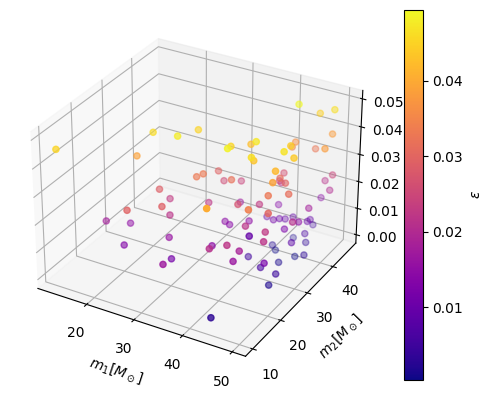
\includegraphics[width=0.45\textwidth]{paper/figures/pop3d_0.05.png}
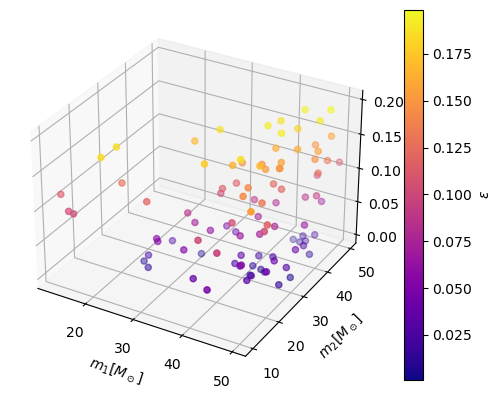
\includegraphics[width=0.45\textwidth]{paper/figures/pop3d_0.2.png}
\caption{\label{fig:pop3d0.05_0.2} Synthetic Population of EBBHs. The left figure represents the population for $\sigma_\epsilon=0.05$ and right figure represents the population for $\sigma_\epsilon=0.2$}
\end{figure*}


%\begin{table*}[]
%    \centering
%    \begin{tabular}{c|cccccc}
%        \hline \hline
%        Populations & $m_{1_{min}} [M_\odot] $ & $m_{1_{max}} [M_\odot]$ & $m_{2_{min}} [M_\odot]$ & $m_{2_{max}} [M_\odot]$ & $\epsilon_{min}$ & $\epsilon_{max}$\\ \hline
%        First  & 12.19 & 49.89 & 10.17 & 46.67 & 0.0004 & 0.0494\\ \hline
%        Second  & 15.42 & 49.79 & 10.46 & 47.59 & 0.0003 & 0.0999\\ \hline
%        Third  & 16.17 & 49.83 & 10.69 & 47.52 & 0.0002 & 0.148\\ \hline
%        Forth  & 12.52 & 49.89 & 10.08 & 49.51 & 0.0012 & 0.1984\\ \hline
%    \end{tabular}
%    \caption{Population Properties of EBBHs}
%    \label{tab:pop_prop}
%\end{table*}

To make our study more realistic, we must add the measurement error in each source.  Rather than generate synthetic gravitational wave sources and perform full Bayesian inference, following previous work \cite{Mandel_2017_Errors} we generate mock measurement errors motivated by real parameter inference investigations. The chirp mass and symmetric mass ratio are well-constrained compared to the primary and secondary masses of BBHs. Therefore, we compute them for each event in a population by using the following relations.

\begin{equation}
    M_c^T = \frac{(m_1 m_2)^{3/5}}{(m_1+m_2)^{1/5}},
\end{equation}

\begin{equation}
    \eta^T = \frac{(m_1 m_2)}{(m_1+m_2)^2},
\end{equation}
%
where $M_c^T$ and $\eta^T$ are found using the primary and secondary masses of each event generated by the power law model.
Furthermore, using the following relations, We add the measurement errors in the $M_c^T$ and $\eta^T$.

\begin{equation}
    M_c = M_c^T\left( 1+\alpha (r_0+r ) \frac{12}{\rho}\right),
\end{equation}

\begin{equation}
\eta = \eta^T\left( 1+0.03 (r_0'+r') \frac{12}{\rho}\right),   
\end{equation}
where $r_0$ and $r_0'$ are the random numbers drawn from the standard normal distribution, which will shift the mean of the $M_c$ and $\eta$ distribution with respect to $M_c^T$ and $\eta^T$. The $r$ and $r'$ are the independent and identically distributed arrays of those randomly generated numbers to spread the distribution. The measurement uncertainty is inversely proportional to signal-to-noise ratio $\rho$, drawn from the distribution $p(\rho) \propto \rho^{-4}$, which holds for isotropically distributed sources in a static universe, subject to the threshold $\rho\geq 8$ for detection. The $\alpha =0.1$ is used for the scaling inspired by analyses of mock data with the LALINFERENCE pipeline \cite{alpha_error_2015} and includes the impact of correlation with parameters describing arbitrary remnant spins.

Finally, after adding the measurement errors in the $M_c$ and $\eta$, we will convert them back to $m_1$ and $m_2$ to perform our analysis. We used the following relation for conversion, and it will provide the masses based on the condition $m_1\geq m_2$.
%
\begin{align}
    m_1 = \frac{1}{2} M_c \eta^{-3/5} (1+\sqrt{\eta_v}), \\
    m_2 = \frac{1}{2} M_c \eta^{-3/5} (1-\sqrt{\eta_v}), 
\end{align}
where $\eta_v = 1-4\eta$, we kept the samples with non-negative values and ignored the negative samples to avoid the square root issues. 

We also added the absolute error in the eccentricity by using the truncated normal distribution scaling at $0.05$ to keep the eccentricity positive.
\textbf{this is important - refer to other papers.  THIS IS REASONABLE FOR LOW MASS BUT VERY OPTIMISTIC FOR HIGH MASS}
STRETCH GOAL: what if you ran again, but with large error?








\subsection{Synthetic population without eccentricity}

To compare the synthetic EBBHs population with the non-eccentric BBHs (NEBBHS), we estimate how our sources would be characterized by parameter inferences which omitted the effects of eccentricity.  Following \cite{favata-scaling-2022}, the following effective chirp mass is well-constrained by observations dominated by the inspiral of a slightly eccentric binary:
\begin{align}
\label{eq:scaling}
M^{ecc} = \frac{M}{(1-\frac{157}{24}\epsilon^2)^{3/5}}
\end{align}
%
Our ansatz for source identification and characterization is that the best-fitting parameters and posteriors are directly related to the true posteriors, except that the recovered chirp mass is given by  Eq. \ref{eq:scaling}.  This process removes the eccentric component from the population only by scaling the masses and omitting the eccentricity. 





%\begin{table*}[]
%    \centering
%    \begin{tabular}{c|cccc}
%        \hline \hline
%        Populations & $m_{1_{min}} [M_\odot] $ & $m_{1_{max}} [M_\odot]$ & $m_{2_{min}} [M_\odot]$ & $m_{_2{max}} [M_\odot]$ \\ \hline
%        First & 12.09 & 49.6 & 10.17 & 46.27 \\ \hline
%        Second & 15.26 & 49.77 & 10.3 & 47.56 \\ \hline
%        Third & 15.96 & 49.5 & 10.62 & 46.60  \\ \hline
%        Forth & 11.86 & 49.76 & 9.67 & 46.99  \\ \hline
%    \end{tabular}
%    \caption{Population Properties of NEBBHs}
    \label{tab:popscl_prop}
%\end{table*}
 

\begin{figure*}

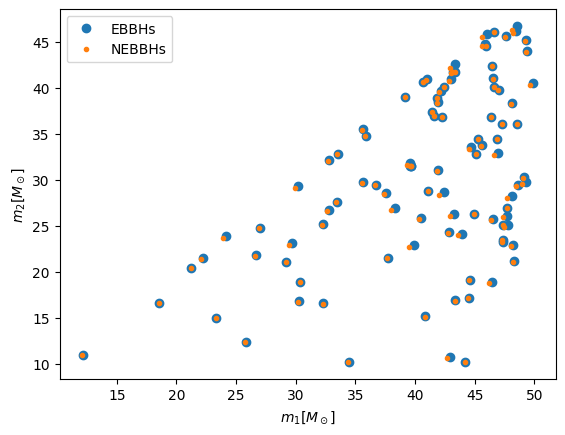
\includegraphics[width=0.45\textwidth]{paper/figures/pop2d_0.05.png}
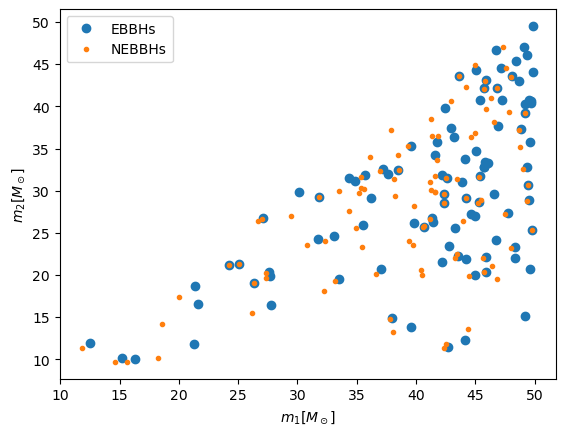
\includegraphics[width=0.45\textwidth]{paper/figures/pop2d_0.2.png}
\caption{\label{fig:pop2d_0.05_0.2} The left figure shows the primary mass vs secondary mass of the EBBHs and NEBBHs with $\sigma_\epsilon =0.05$. The right figure shows the same plot but for $\sigma_\epsilon=0.2$} 

\end{figure*}

   


The significant effect after scaling is the mass shift, which can be observed in Fig. \ref{fig:pop2d_0.05_0.2}. In this figure, the left-hand side shows the mass shift of the first population generated with smaller $\sigma_\epsilon =0.05$, which leads to a lesser mass shift. However, on the right hand of Fig. \ref{fig:pop2d_0.05_0.2}, one can see the significant mass shift after removing the eccentric component.  This also reflects that we may miss the various sources by ignoring the effect of eccentricity and we notice that sources start missing, which has eccentricity $\epsilon>0.38$.


                            

\section{Population Inference}
\label{sec:pop_inference}
We have use the prior's given in the table \ref{tab:prior}

\begin{table*}
    \centering
    \begin{tabular}{c|ccccc}
        \hline \hline
       Quantity & $\log_{10}(\frac{\mathcal{R}}{\rm Gpc^{-3}yr^{-1}})$ & $\alpha$ & $m_{min} [M_\odot] $ & $m_{max} [M_\odot]$ & $\sigma_\epsilon$ \\ \hline
      Synthetic population & 2 & -1 & 10 & 50 & 0.05-0.2 \\ \hline
      Prior range & $[-3,3]$ & $[-5,5]$ & $[1-20]$ & $[30-80]$ & $[0-0.5]$ \\ \hline
      Prior distribution & Log-uniform & Uniform & Uniform & Uniform & Uniform  \\ \hline \hline
    \end{tabular}
    \caption{Parameter used to generate synthetic population and prior used for the inference}
    \label{tab:prior}
\end{table*}


Figure A shows the results of population inference under the most conservative case with $\sigma_\epsilon=0.05$.  In this figure, the ZZ color shows the results of QQ.
%
Most notably, this figure shows that even in the limit of extremely small ecctricity, the impact of eccentricity can be measured from a large population of observations, comparable to the current size.  This result depends of course on our assumption that all binaries are equally likely to have eccentricity, and that our measurement uncertainty in eccentricity is both indpeendent of mass and fairly small, both optimisitic assumptions.  In fact, the overall uncertainty in $\sigma_\epsilon$ is expected: given 100 events, each with a measurement error of $0.05$, we expect $\sigma_\epsilon$ to be measured to of order $0.05/\sqrt{N}$ (handwavy -- really a chisquared distribution,etc).
SUSPECT THAT IF YOU MAKE THIS JUST 3X bigger, STILL GET RESULT -- you will almost always get this result

Also noteworthy is the impact of neglecting eccentricity.  If eccentricity is neglected, then the population inference is biased away from true values: the black contours in the first column do not include the true values for $m_{max}, m_{min}$ example.



Figure B shows the results of population inference under the most optimistic case with $\sigma_\epsilon=0.2$.  In this figure, the ZZ color shows the results of QQ.


we can discuss the corner plots here.

TAKEAWAYS

* Eccentricity can be measured

* If not measured, biases




\begin{figure*}

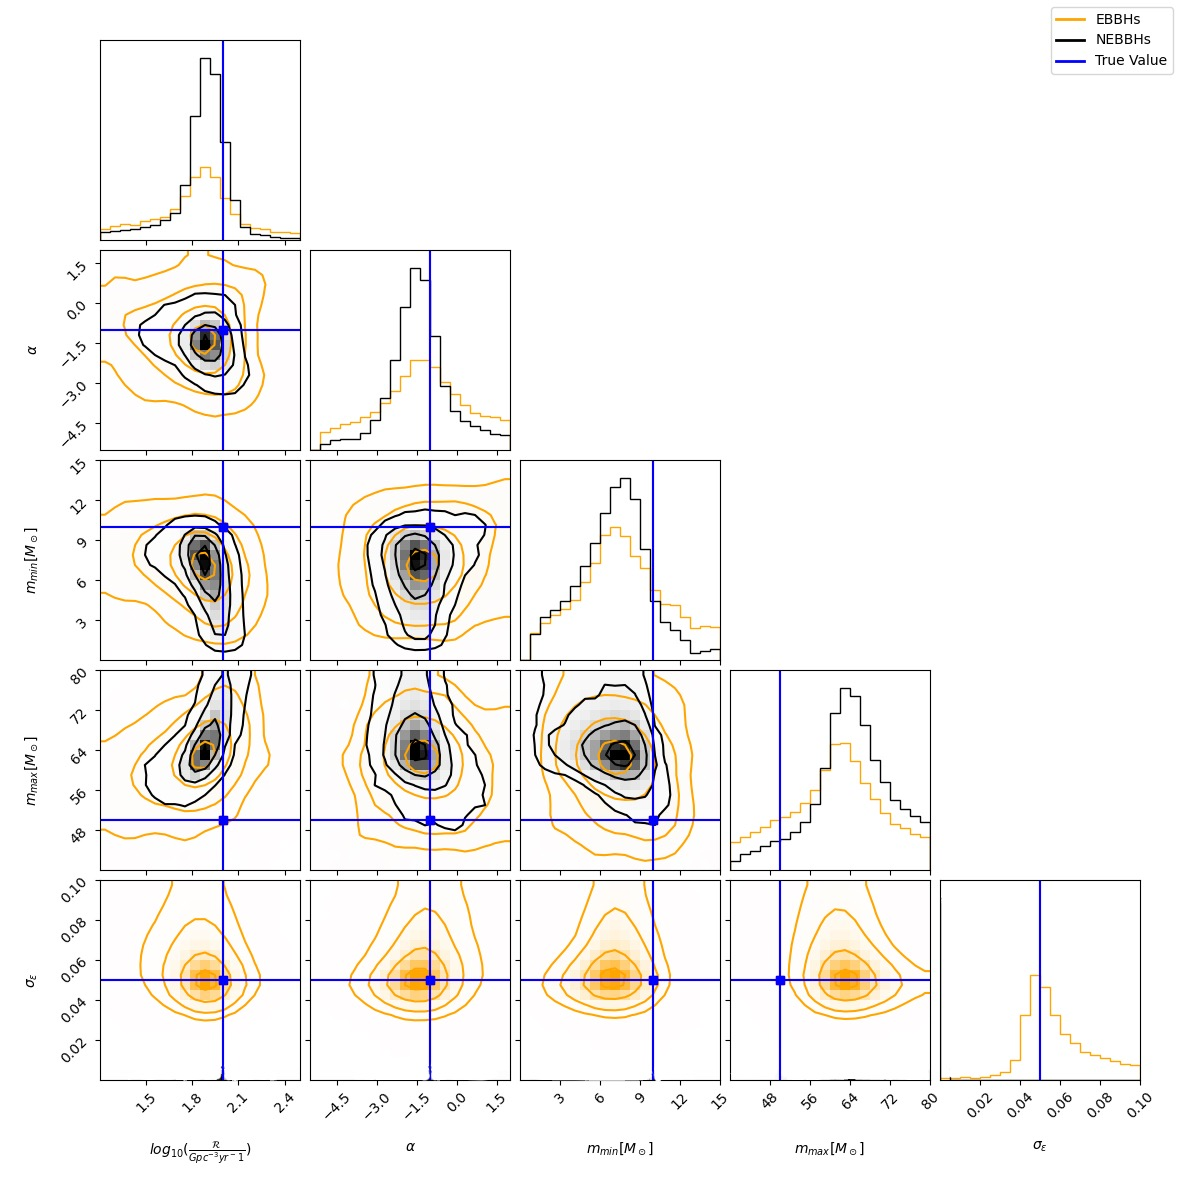
\includegraphics[width=0.95\textwidth]{paper/figures/cor_0.05.png}
\caption{\label{fig:pop3d05}\textbf{Corner Plots for EBBHs and BBHS for $\sigma_\epsilon=0.05$}}

\end{figure*}

\begin{figure*}

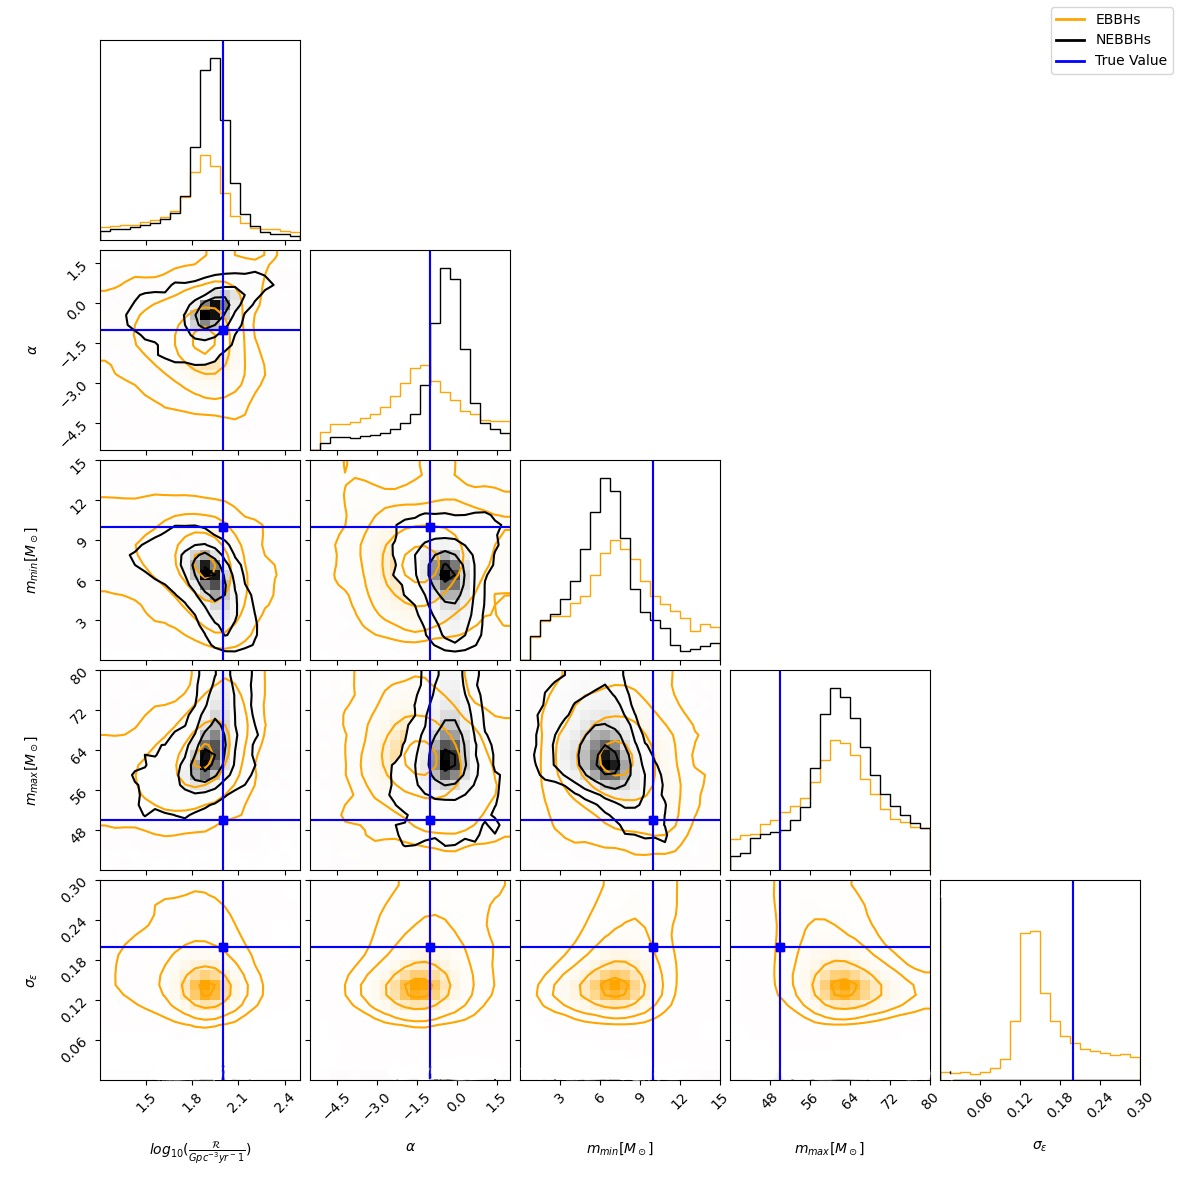
\includegraphics[width=0.95\textwidth]{paper/figures/cor_0.2.png}
\caption{\label{fig:pop3d05}\textbf{Corner Plots for EBBHs and BBHs for $\sigma_\epsilon=0.2$}}

\end{figure*} 

%\renewcommand{\arraystretch}{2}
\begin{table*}
    \centering
    \begin{tabular}{c|ccccc}
        \hline \hline
       Inference & $log_{10}(\frac{\mathcal{R}}{Gpc^{-3}yr^-1})$ & $\alpha$ & $m_{min} [M_\odot] $ & $m_{max} [M_\odot]$ & $\sigma_\epsilon$ \\ \hline
      First& $1.42^{+0.58}_{-2.64}$ & $-0.88^{+3.17}_{-1.89}$ & $8.36^{+7.49}_{-3.51}$ & $58.44^{+10.21}_{-24.31}$ & $0.30^{+0.54}_{-0.25}$ \\ \hline
      Second & $1.36^{+0.63}_{-2.65}$ & $-0.93^{+3.29}_{-1.92}$ & $8.71^{+7.36}_{-3.81}$ & $57.84^{+10.81}_{-25.53}$ & $0.33^{+0.51}_{-0.25}$ \\ \hline
      Third & $1.39^{+0.58}_{-2.69}$ & $-0.69^{+2.98}_{-1.95}$ & $9.21^{+6.31}_{-3.99}$ & $57.85^{+10.73}_{-27.04}$ & $0.33^{+0.51}_{-0.23}$  \\ \hline
      Forth & $1.27^{+0.72}_{-2.68}$ & $-0.90^{+3.30}_{-1.98}$ & $8.63^{+7.85}_{-3.72}$ & $57.76^{+11.03}_{-25.82}$ & $0.37^{+0.47}_{-0.23}$  \\ \hline \hline
    \end{tabular}
    \caption{Population Inference for EBBHs}
    \label{tab:inference_EBBHS}
\end{table*}


\begin{table*}[]
    \centering
    \begin{tabular}{c|cccc}
        \hline \hline
        Inference & $log_{10}(\frac{\mathcal{R}}{Gpc^{-3}yr^-1})$ & $\alpha$ & $m_{min} [M_\odot] $ & $m_{max} [M_\odot]$ \\ \hline
      First & $1.85^{+0.14}_{-1.23}$ & $-1.37^{+1.43}_{-0.94}$ & $7.54^{+3.68}_{-3.04}$ & $63.29^{+8.00}_{-13.08}$  \\ \hline
      Second & $1.83^{+0.14}_{-1.38}$ & $-1.12^{+1.47}_{-0.91}$ & $7.69^{+3.88}_{-3.15}$ & $61.91^{+8.59}_{-13.87}$  \\ \hline
      Third & $1.84^{+0.15}_{-1.55}$ & $-0.38^{+1.03}_{-0.96}$ & $8.07^{+3.44}_{-3.27}$ & $61.70^{+8.49}_{-24.26}$   \\ \hline
      Forth & $1.86^{+0.16}_{-1.85}$ & $-0.31^{+1.17}_{-1.14}$ & $6.99^{+8.77}_{-2.58}$ & $61.15^{+8.72}_{-16.84}$  \\ \hline \hline
    \end{tabular}
    \caption{Population Inference for NEBBHs}
    \label{tab:inference_NEBBHS}
\end{table*}






\section{Conclusions}
\label{sec:conclude}
In Progress, 




* summarize your calculations

* summarize key takeaways

** we WILL find this, measuremeent error can't be too large/infinite!

* contrast /compare with other papers 

* some comments on what it all means for the big picture (dynamical evolution tests for example could be done)



The first potential reason for getting circular orbits is that eccentric effects are more evident in low-mass events, and current searches are more efficient for higher-mass mergers. Secondly, it may result from selection biases in the waveforms because LVK detectors only use circular waveforms for parameter estimation (PE), which better present binaries evolved in an isolated environment.


Studies show that we must consider the multiple formation channels to understand the population better. Because a single channel does not contribute more than $70\%$ of the observation sample of BBHs \cite{zevin-2021} \textbf{previous statement speculative/unsupported - remove}.

which leads towards the dynamical formation of the source. So, it is critical for astrophysical implications to assess eccentricity distribution


We may also have stellar mass higher eccentric mergers at the lower frequency searches \cite{sesana-2016,chen-2017}, which can be measurable by detectors like Laser Interferometer Space Antenna (LISA) \cite{LISA-2017}. These observations would allow for long-term tracking of BBHs orbital properties, which can be used to infer the formation mechanism \cite{Breivik-2016}.

The sensitivity of LVK detectors is increasing with time, leading to more detection in each observing run. We will have hundreds of events in future runs, and with the upcoming O4 run, we expect detection every other day \cite{detection_rate_2016,detection_rate_2015}. 
Interestingly, the new detections lead us to the reasonable disagreement on the masses, spin, event rate, and formation scenarios \cite{LSC-BBH-2016, LSC-GW150914-2016}, which pushes researchers to develop new models \cite{Mandel-2016,marchant-2016}, and also provide more information about the observable GWs \cite{Barausse-2018, Abbot-2016-schotastic,dvorkin-2016}. Therefore, identifying and understanding the populations of EBBHs with a growing number of detection will give us more insightful information about the formation and evolution of massive stars from birth to death over cosmic time.


\begin{acknowledgements}
We thank our anonymous referee for the helpful feedback.

\end{acknowledgements}


%\appendix
%In Progress,




%\bibstyle{unsrt}
\bibliography{paperexport,LIGO-publications}
\end{document}
